\documentclass[handout]{beamer}  
%use [handout] option to print without all the pauses!
\usepackage{setspace}
\linespread{1.3}
\usepackage{amssymb, amsmath, amsthm} 
\usepackage{rotating}
\usepackage{multirow}
\usepackage{graphicx}
\usepackage{enumerate}
\usepackage{synttree}
\usepackage{fancybox}
\usepackage{color}
\usepackage{tikz}
\usetikzlibrary{trees}
\newcommand{\p}{\mathbb{P}}
\newcommand{\expect}{\mathbb{E}}
\newcommand{\var}{\mathbb{V}}



%\setbeamertemplate{blocks}[rounded][shadow=true] 
%gets rid of bottom navigation bars
\setbeamertemplate{footline}{
   \begin{beamercolorbox}[ht=4ex,leftskip=0.3cm,rightskip=0.3cm]{author in head/foot}
%    \usebeamercolor{UniBlue}
    \vspace{0.1cm}
    %\insertshorttitle \ - \insertdate 
    \hfill \insertframenumber / \inserttotalframenumber
   \end{beamercolorbox}
   \vspace*{0.1cm}
} 

%gets rid of navigation symbols
\setbeamertemplate{navigation symbols}{}


%Include or exclude the notes?
%\setbeameroption{show notes}
\setbeameroption{hide notes}


\title[Econ 103]{Economics 103, Statistics for Economists} 
\author[F. DiTraglia]{Francis J.\ DiTraglia}
\institute{University of Pennsylvania}
\date{Lecture 18}


\begin{document} 




%%%%%%%%%%%%%%%%%%%%%%%%%%%%%%%%%%%%%%%%

\begin{frame}[plain]
	\titlepage 
	

\end{frame} 



%%%%%%%%%%%%%%%%%%%%%%%%%%%%%%%%%%%%%%%%
%\begin{frame}
%\frametitle{General Procedure for Finding Confidence Intervals}
%Suppose we have an estimator $\widehat{\theta}$ of a population parameter $\theta_0$. Our goal is to construct an interval $(A,B)$ such that
%	$$\p(A \leq \theta_0 \leq B) = 1-\alpha$$
%	\begin{enumerate}[Step 1]
%\item Find an expression involving $\widehat{\theta}$ and $\theta_0$, call it $T(\widehat{\theta}, \theta_0)$ with a \emph{known sampling distribution G}. \pause
%\item Use the quantile function of $G$ to find $\ell, u$ such that $\p[\ell \leq T(\widehat{\theta}, \theta_0) \leq u] = 1-\alpha$. \pause 
%\item Manipulate $\p[\ell \leq T(\widehat{\theta}, \theta_0) \leq u] = 1-\alpha$ to get $\theta_0$ by itself in the middle. 
%\end{enumerate}
%\end{frame}

%%%%%%%%%%%%%%%%%%%%%%%%%%%%%%%%%%%%%%%%
\begin{frame}
\frametitle{Two-sample Problem \hfill 
\includegraphics[scale = 0.05]{./images/clicker}}
Suppose $X_1, \hdots, X_{n} \sim \mbox{iid } N(\mu_x, \sigma^2_x)$ independently of $Y_1, \hdots, Y_{m} \sim \mbox{iid } N(\mu_y, \sigma^2_y)$. What is \alert{$\expect[\bar{X}_n - \bar{Y}_m]$}, the expectation of the sampling distribution of the difference of sample means?

\begin{enumerate}[(a)]
	\item $\mu_x$
	\item $\mu_x - \mu_y$
	\item $\mu_y$
	\item $\mu_x + \mu_y$
	\item 0
\end{enumerate}

\pause
\vspace{1em} 

\alert{$\expect[\bar{X}_n - \bar{Y}_m] = \pause \expect[\bar{X}_n] - \expect[\bar{Y}_m] =\pause \mu_x - \mu_y$}
\end{frame}
%%%%%%%%%%%%%%%%%%%%%%%%%%%%%%%%%%%%%%%%
\begin{frame}
\frametitle{Two-sample Problem \hfill 
\includegraphics[scale = 0.05]{./images/clicker}}
Suppose $X_1, \hdots, X_{n} \sim \mbox{iid } N(\mu_x, \sigma^2_x)$ independently of $Y_1, \hdots, Y_{m} \sim \mbox{iid } N(\mu_y, \sigma^2_y)$. What is \alert{$Var[\bar{X}_n - \bar{Y}_m]$}, the variance of the sampling distribution of the difference of sample means?

\begin{enumerate}[(a)]
	\item $\sigma_x^2 - \sigma_y^2$
	\item $\sigma_x^2 + \sigma_y^2$
	\item $\sigma_x^2/n + \sigma_y^2/m$
	\item $\sigma_x^2/n - \sigma_y^2/m$
	\item 1
\end{enumerate}

\pause
\vspace{1em} 

\alert{By independence: $Var[\bar{X}_n - \bar{Y}_m] =\pause Var[\bar{X}_n] + Var[\bar{Y}_m] = \pause \displaystyle \frac{\sigma_x^2}{n} + \frac{\sigma_y^2}{m}$}
\end{frame}
%%%%%%%%%%%%%%%%%%%%%%%%%%%%%%%%%%%%%%%%
\begin{frame}
\frametitle{Two-sample Problem \hfill 
\includegraphics[scale = 0.05]{./images/clicker}}
Suppose $X_1, \hdots, X_{n} \sim \mbox{iid } N(\mu_x, \sigma^2_x)$ independently of $Y_1, \hdots, Y_{m} \sim \mbox{iid } N(\mu_y, \sigma^2_y)$. What is the \alert{sampling distribution} of $\bar{X}_n - \bar{Y}_m$, the difference of sample means?

\begin{enumerate}[(a)]
	\item $\chi^2$
	\item $t$
	\item $F$
	\item Normal
\end{enumerate}

\pause
\vspace{1em}

\alert{Normal, by independence and linearity property of normal distributions.}
\end{frame}
%%%%%%%%%%%%%%%%%%%%%%%%%%%%%%%%%%%%%%%%
\begin{frame}
\frametitle{Sampling Distribution of $\bar{X}_n - \bar{Y}_m$}
Suppose $X_1, \hdots, X_{n} \sim \mbox{iid } N(\mu_x, \sigma^2_x)$ independently of $Y_1, \hdots, Y_{m} \sim \mbox{iid } N(\mu_y, \sigma^2_y)$. Then,
	$$\left(\bar{X}_n - \bar{Y}_m\right) \sim N \left( \mu_x - \mu_y, \frac{\sigma_x^2}{n} + \frac{\sigma_y^2}{m} \right) $$
	
\pause

$$\alert{\frac{\left(\bar{X}_n - \bar{Y}_m\right) - (\mu_x - \mu_y)}{\sqrt{\displaystyle\frac{\sigma_x^2}{n} + \frac{\sigma_y^2}{m} }}\sim N(0,1)}$$
\pause

Shorthand: $SE(\bar{X}_n - \bar{Y}_m) = \sqrt{\displaystyle\frac{\sigma_x^2}{n} + \frac{\sigma_y^2}{m} }$

\end{frame}
%%%%%%%%%%%%%%%%%%%%%%%%%%%%%%%%%%%%%%%%
\begin{frame}
\frametitle{CI for Difference of Population Means, $\sigma_x^2, \sigma_y^2$ Known}
	$$\frac{(\bar{X}_n - \bar{Y}_m) - (\mu_x -\mu_y)}{SE(\bar{X}_n - \bar{Y}_m)} \sim N(0,1)$$
	
	\vspace{1em}

Thus, we construct a $100\times(1-\alpha)\%$ CI for $\mu_x - \mu_y$ as follows:
	$$\alert{(\bar{X}_n - \bar{Y}_m) \pm \; \texttt{qnorm}(1-\alpha/2) \; SE(\bar{X}_n - \bar{Y}_m)}$$
Where $SE(\bar{X}_n - \bar{Y}_m) = \sqrt{\displaystyle\frac{\sigma_x^2}{n} + \frac{\sigma_y^2}{m} }$
\end{frame}
%%%%%%%%%%%%%%%%%%%%%%%%%%%%%%%%%%%%%%%%
\begin{frame}
\frametitle{Calculate the SE for the Difference of Means \hfill 
\includegraphics[scale = 0.05]{./images/clicker}}
I generated independent random samples of size 25 from two normal distributions in R. One had a population standard deviation of 4 and the other had a population standard deviation of 3. The sample means were approximately 4.2 and 3.1.

\vspace{1em}
\alert{Calculate the ME for a 95\% confidence interval for the difference of population means.}

\pause
\begin{eqnarray*}
	SE &=& \sqrt{\frac{3^2}{25} + \frac{4^2}{25}} = \frac{\sqrt{9 + 16}}{5} = 1\\  \\\pause
	ME &=& \texttt{qnorm(1 - 0.05/2)} \times SE \approx 2 \times SE = 2
\end{eqnarray*}

\end{frame}
%%%%%%%%%%%%%%%%%%%%%%%%%%%%%%%%%%%%%%%%
\begin{frame}
\frametitle{Calculate the SE for the Difference of Means \hfill 
\includegraphics[scale = 0.05]{./images/clicker}}
I generated independent random samples of size 25 from two normal distributions in R. One had a population standard deviation of 4 and the other had a population standard deviation of 3. The sample means were approximately 4.2 and 3.1.

\vspace{1em}
\alert{Calculate the LCL for a 95\% confidence interval for the difference of population means.}
\pause
$$LCL = (4.2 - 3.1) - ME = 1.1 - 2 = -0.9$$
\end{frame}
%%%%%%%%%%%%%%%%%%%%%%%%%%%%%%%%%%%%%%%%

\begin{frame}
\frametitle{Calculate the UCL for the Difference of Means \hfill 
\includegraphics[scale = 0.05]{./images/clicker}}
I generated independent random samples of size 25 from two normal distributions in R. One had a population standard deviation of 4 and the other had a population standard deviation of 3. The sample means were approximately 4.2 and 3.1.

\vspace{1em}
\alert{Calculate the UCL for a 95\% confidence interval for the difference of population means.}\pause

$$UCL = (4.2 - 3.1) + ME =1.1 + 2 = 3.1$$

\pause

\alert{$$\boxed{95\% \mbox{ Confidence Interval: } (-0.9, 3.1)}$$} \pause
The actual population means were 4 and 3, respectively
\end{frame}
%%%%%%%%%%%%%%%%%%%%%%%%%%%%%%%%%%%%%%%%


\begin{frame}
\frametitle{What if $\sigma_x^2,\sigma_y^2$ are Unknown?}
Suppose $X_1, \hdots, X_{n} \sim \mbox{iid } N(\mu_x, \sigma^2_x)$ independently of $Y_1, \hdots, Y_{m} \sim \mbox{iid } N(\mu_y, \sigma^2_y)$. Then,

\vspace{1em}
$$\frac{\left(\bar{X}_n - \bar{Y}_m\right) - (\mu_x - \mu_y)}{\sqrt{\displaystyle\frac{S_x^2}{n} + \frac{S_y^2}{m} }}\sim t(\nu)$$
\vspace{1em}

\begin{block}{Formula for $\nu$ is Complicated and You Don't Need to Know it}
Two possibilities:
	\begin{enumerate}
		\item Have R find the correct value of $\nu$ for us
		\item If $m,n$ are large enough, approximately standard normal. 
	\end{enumerate}
\end{block}

\end{frame}
%%%%%%%%%%%%%%%%%%%%%%%%%%%%%%%%%%%%%%%%
\begin{frame}
\frametitle{Case of Equal, Unknown Variances}

The book considers a case where $\sigma^2_x = \sigma^2_y = \sigma^2$, that is a common unknown variance. This is a \alert{very dangerous assumption}. It is almost certainly false and can throw off our results in a serious way. You are not responsible for this case.
\end{frame}
%%%%%%%%%%%%%%%%%%%%%%%%%%%%%%%%%%%%%%%%

\begin{frame}
\frametitle{Sampling Distributions Under Normality: One-sample}
Suppose that $X_1, \hdots, X_n \sim \mbox{iid } N(\mu,\sigma^2)$. Then:

	\begin{eqnarray*}
		\left(\frac{n-1}{\sigma^2}\right) S^2&\sim&\chi^2(n-1)\\ \\
		\frac{\bar{X}_n-\mu}{\sigma/\sqrt{n}}&\sim& N(0,1)\\ \\
		\frac{\bar{X}_n-\mu}{S/\sqrt{n}}&\sim&t(n-1)
	\end{eqnarray*}
\end{frame}
%%%%%%%%%%%%%%%%%%%%%%%%%%%%%%%%%%%%%%%%
\begin{frame}
\frametitle{Sampling Distributions Under Normality: Two-sample}
Suppose $X_1, \hdots, X_{n} \sim \mbox{iid } N(\mu_x, \sigma^2_x)$ independently of $Y_1, \hdots, Y_{m} \sim \mbox{iid } N(\mu_y, \sigma^2_y)$. Then:


	\begin{eqnarray*}
\frac{(\bar{X}_n - \bar{Y}_n) - (\mu_x -\mu_y)}{\sqrt{\displaystyle\frac{\sigma_x^2}{n} + \frac{\sigma_y^2}{m} }} &\sim& N(0,1) \\ \\ \\
		\frac{\left(\bar{X}_n - \bar{Y}_m\right) - (\mu_x - \mu_y)}{\sqrt{\displaystyle\frac{S_x^2}{n} + \frac{S_y^2}{m} }}&\sim& t(\nu)
	\end{eqnarray*}
\end{frame}
%%%%%%%%%%%%%%%%%%%%%%%%%%%%%%%%%%%%%%%%

\begin{frame}
\begin{center}\Huge But what if the population isn't Normal?\end{center}
\end{frame}

%%%%%%%%%%%%%%%%%%%%%%%%%%%%%%%%%%%%%%%%
\begin{frame}
\frametitle{The Central Limit Theorem}
Suppose that $X_1, \hdots, X_n$ are a random sample from a population with unknown mean $\mu$. Then, provided that $n$ is \alert{\emph{sufficiently large}}, the sampling distribution of $\bar{X}_n$ is approximately $N\left(\mu, \widehat{SE}(\bar{X}_n)^2\right)$, even if the even if the underlying population is \alert{non-normal}.

\begin{block}{In Other Words...}
	$$\frac{\bar{X}_n -\mu}{\widehat{SE}(\bar{X}_n)} \approx N(0,1)$$
\end{block}

\begin{alertblock}{Use this to create \emph{approximate} CIs for population mean!}
\end{alertblock}
\end{frame}
%%%%%%%%%%%%%%%%%%%%%%%%%%%%%%%%%%%%%%%%
\begin{frame}
\begin{center}\Huge You should be amazed by this.\end{center}
\end{frame}
%%%%%%%%%%%%%%%%%%%%%%%%%%%%%%%%%%%%%%%%
\begin{frame}
\frametitle{Example: Uniform(0,1) Population, $n = 20$}
\begin{figure}
\centering
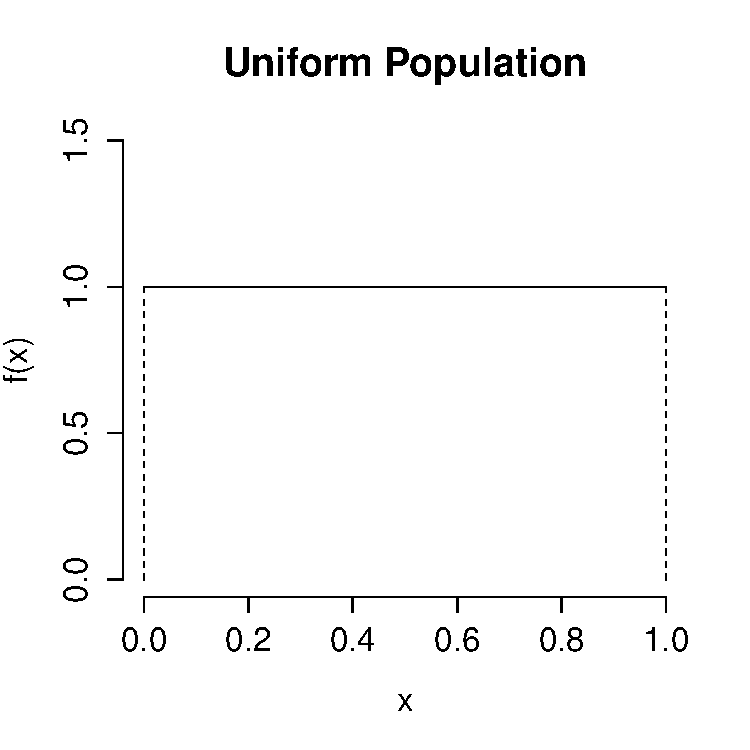
\includegraphics[scale = 0.4]{./images/uniform_pdf}
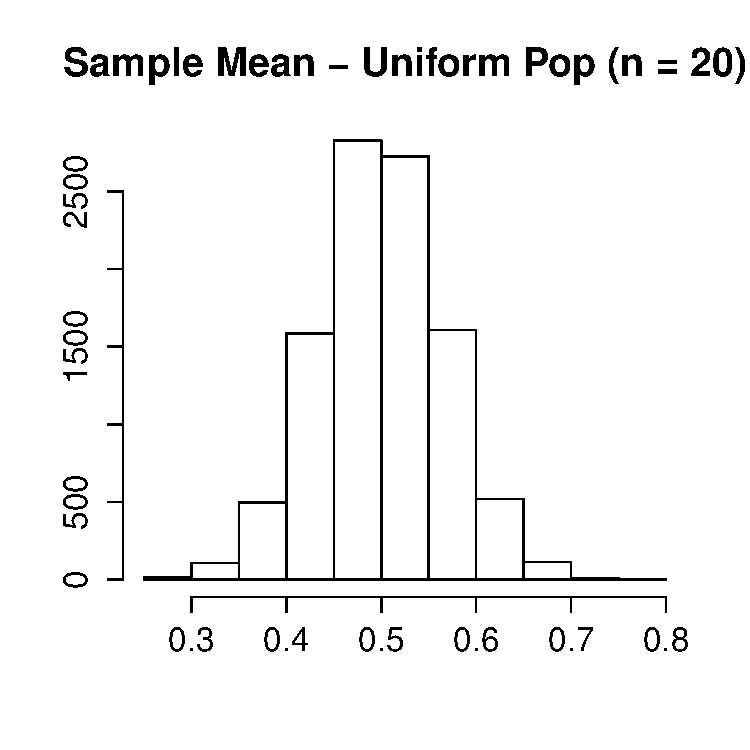
\includegraphics[scale = 0.4]{./images/xbar_uniform}
\end{figure}
\end{frame}
%%%%%%%%%%%%%%%%%%%%%%%%%%%%%%%%%%%%%%%%
\begin{frame}
\frametitle{Example: $\chi^2(5)$ Population, $n = 20$}
\begin{figure}
\centering
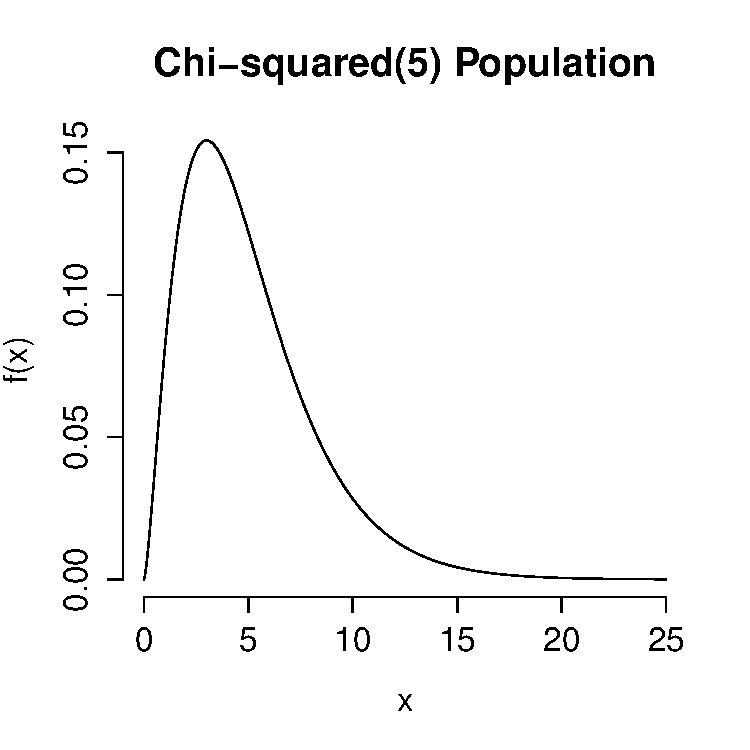
\includegraphics[scale = 0.4]{./images/chisq_pop}
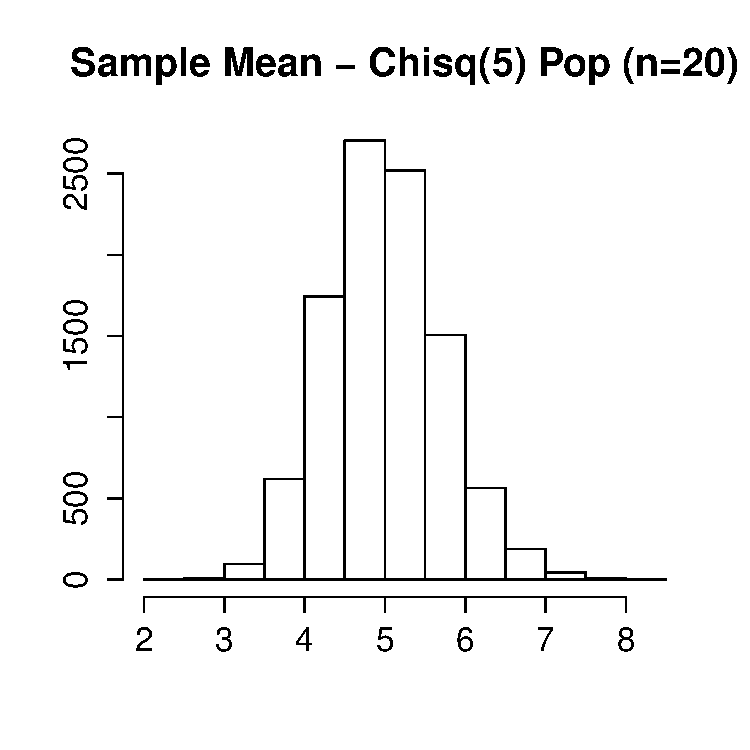
\includegraphics[scale = 0.4]{./images/xbar_chisq}
\end{figure}
\end{frame}
%%%%%%%%%%%%%%%%%%%%%%%%%%%%%%%%%%%%%%%%
\begin{frame}
\frametitle{Example: Bernoulli$(0.3)$ Population, $n =20$}
\begin{figure}
\centering
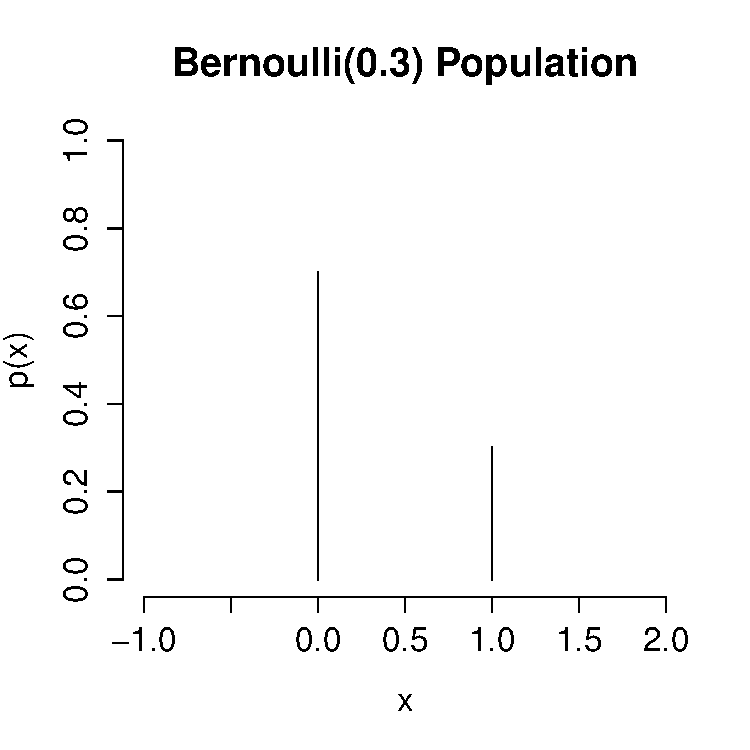
\includegraphics[scale = 0.4]{./images/bernoulli}
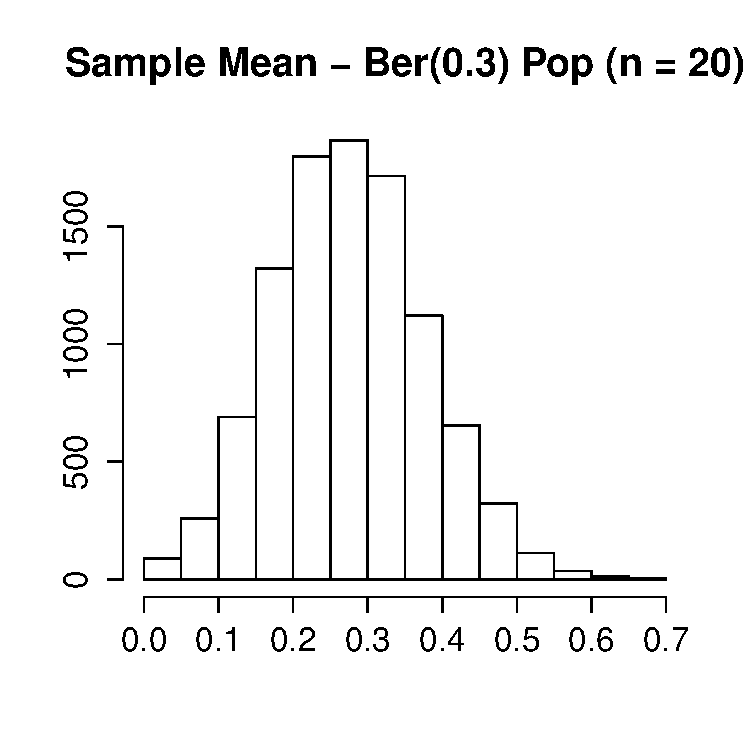
\includegraphics[scale = 0.4]{./images/xbar_bernoulli}
\end{figure}
\end{frame}
%%%%%%%%%%%%%%%%%%%%%%%%%%%%%%%%%%%%%%%%

\begin{frame}
\frametitle{Who is the Chief Justice of the US Supreme Court?\hfill 
\includegraphics[scale = 0.05]{./images/clicker}}
	\begin{enumerate}[(a)]
	\item Harry Reid
	\item John Roberts
	\item William Rehnquist
	\item Stephen Breyer
\end{enumerate}

% \vspace{1em}
% \alert{58/65 $\approx 90\%$ of the students in the class got this right. }

\end{frame}
%%%%%%%%%%%%%%%%%%%%%%%%%%%%%%%%%%%%%%%%
\begin{frame}
\frametitle{Are US Voters Really That Ignorant?}
\framesubtitle{\fbox{\href{http://www.people-press.org/files/2012/08/8-10-12-Knowledge-release.pdf}{Pew: ``What Voters Know About Campaign 2012''}}}

\begin{block}{The Data}
Of 771 registered voters polled, only 39\% correctly identified John Roberts as the current chief justice of the US Supreme Court.
\end{block}

\begin{block}{Research Question}
Is the majority of voters unaware that John Roberts is the current chief justice, or is this just sampling variation?
\end{block}

\alert{Assume Random Sampling...}

\end{frame}
%%%%%%%%%%%%%%%%%%%%%%%%%%%%%%%%%%%%%%%%
\begin{frame}
\frametitle{Confidence Interval for a Proportion}
	\begin{block}{What is the appropriate probability model for the sample?} 
$X_1, \hdots, X_n \sim \mbox{iid Bernoulli}(p)$, 1 = Know Roberts is Chief Justice
\end{block}

\pause

	\begin{block}{What is the parameter of interest?}
$p$ = Proportion of voters \emph{in the population} who know Roberts is Chief Justice.
\end{block}

\pause

\begin{block}{What is our estimator?} 
Sample Proportion: $\widehat{p} = (\sum_{i=1}^n X_i)/n$
\end{block}
\end{frame}
%%%%%%%%%%%%%%%%%%%%%%%%%%%%%%%%%%%%%%%%
\begin{frame}
\frametitle{Sample Proportion \emph{is} the Sample Mean!}
\small
$X_1, \hdots, X_n \sim \mbox{iid Bernoulli}(p)$
		$$\widehat{p} = \frac{1}{n} \sum_{i=1}^n X_i = \bar{X}_n$$

\pause


	\begin{eqnarray*}
		E[\widehat{p}] &=&  E\left(\frac{1}{n}\sum_{i=1}^n X_i\right) =  \frac{1}{n} \sum_{i=1}^n E[X_i] =   \frac{np}{n} =  p\\ \\ \pause
		Var(\widehat{p}) &=&  Var\left(\frac{1}{n}\sum_{i=1}^n X_i\right) = \frac{1}{n^2} \sum_{i=1}^n Var(X_i) = \frac{n p(1-p)}{n^2} =  \frac{p(1-p)}{n} \\ \\  \pause
		SE(\widehat{p}) &=&  \sqrt{Var(\widehat{p})} =  \sqrt{\frac{p(1-p)}{n}} \\ \\ \pause
		\widehat{SE}(\widehat{p}) &=&  \sqrt{\frac{\widehat{p}(1-\widehat{p})}{n}}
	\end{eqnarray*}

\end{frame}
%%%%%%%%%%%%%%%%%%%%%%%%%%%%%%%%%%%%%%%%
\begin{frame}
\frametitle{Central Limit Theorem Applied to Sample Proportion}

\begin{alertblock}{Central Limit Theorem: Intuition}
Sample means are approximately normally distributed provided the sample size is large even if the population is non-normal.
\end{alertblock}

\begin{columns}

\column{0.5\textwidth}
\begin{block}{CLT For Sample Mean}
$$\frac{\bar{X}_n -\mu}{\widehat{SE}(\bar{X}_n)} \approx N(0,1)$$
\end{block}

\column{0.5\textwidth}
\begin{block}{CLT for Sample Proportion}
$$\frac{\widehat{p} -p}{\sqrt{\frac{\widehat{p}(1-\widehat{p})}{n}}} \approx N(0,1)$$
\end{block}
\end{columns}

\vspace{1em}
In this example, the population is Bernoulli$(p)$ rather than normal. The sample mean is $\widehat{p}$ and the population mean is $p$.

\end{frame}
%%%%%%%%%%%%%%%%%%%%%%%%%%%%%%%%%%%%%%%%
\begin{frame}
\frametitle{Approximate 95\% CI for Population Proportion}
$$\frac{\widehat{p} -p}{\sqrt{\frac{\widehat{p}(1-\widehat{p})}{n}}} \approx N(0,1)$$ 
	\begin{eqnarray*}
		P\left(-2 \leq\frac{\widehat{p} -p}{\sqrt{\frac{\widehat{p}(1-\widehat{p})}{n}}} \leq  2\right) &\approx& 0.95\\ \\ 
		P\left(\widehat{p} - 2 \sqrt{\frac{\widehat{p}(1-\widehat{p})}{n}} \leq p \leq \widehat{p} + 2\sqrt{\frac{\widehat{p}(1-\widehat{p})}{n}}\right) &\approx& 0.95
	\end{eqnarray*}
\end{frame}



%%%%%%%%%%%%%%%%%%%%%%%%%%%%%%%%%%%%%%%%
\begin{frame}
\frametitle{$100\times(1-\alpha)$ CI for Population Proportion $(p)$}
$X_1, \hdots, X_n \sim \mbox{iid Bernoulli}(p)$
	$$\widehat{p} \pm \texttt{qnorm}(1-\alpha/2) \sqrt{\frac{\widehat{p}(1-\widehat{p})}{n}}$$
	\alert{Approximation based on the CLT. Works well provided $n$ is large and $p$ isn't too close to zero or one.}
\end{frame}
%%%%%%%%%%%%%%%%%%%%%%%%%%%%%%%%%%%%%%%%

\begin{frame}
\frametitle{Example: Bernoulli$(0.9)$ Population, $n =20$}
\begin{figure}
\centering
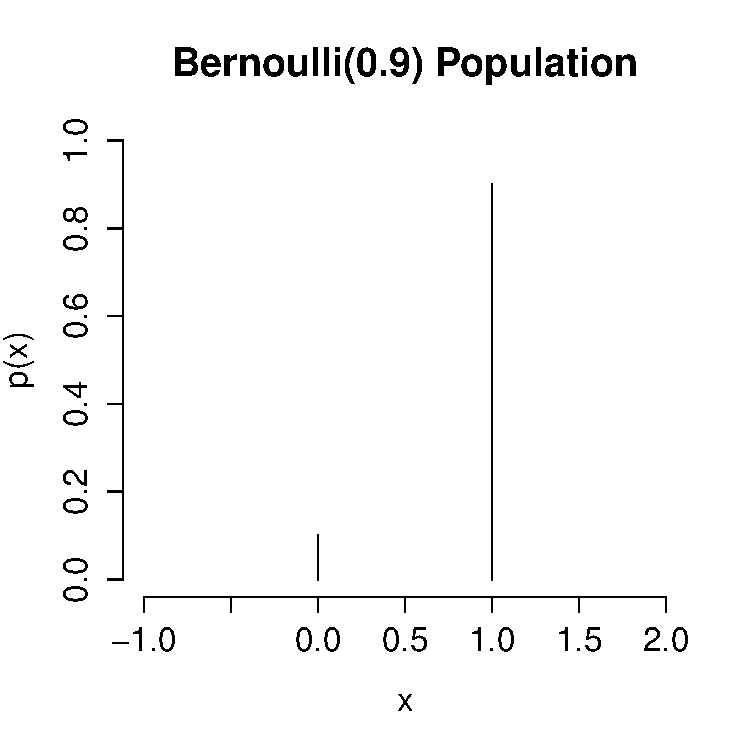
\includegraphics[scale = 0.4]{./images/bernoulli_bad}
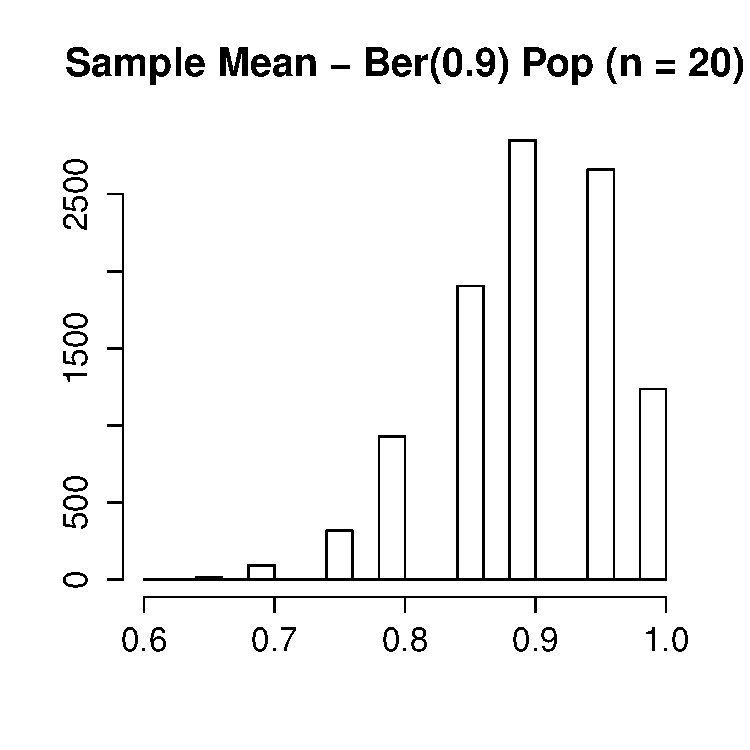
\includegraphics[scale = 0.4]{./images/xbar_bernoulli_bad}
\end{figure}
\end{frame}
%%%%%%%%%%%%%%%%%%%%%%%%%%%%%%%%%%%%%%%%
\begin{frame}
\frametitle{Example: Bernoulli$(0.9)$ Population, $n =100$}
\begin{figure}
\centering
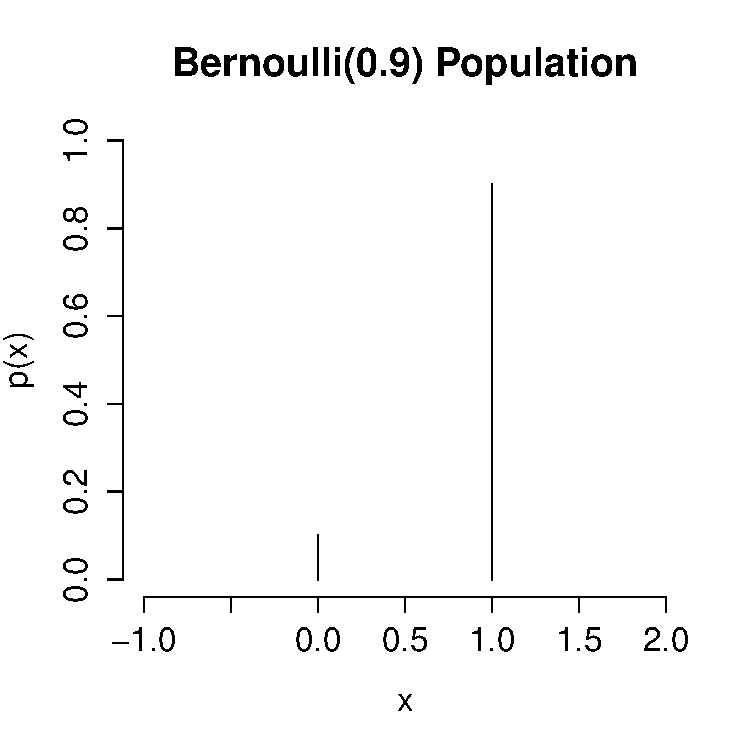
\includegraphics[scale = 0.4]{./images/bernoulli_bad}
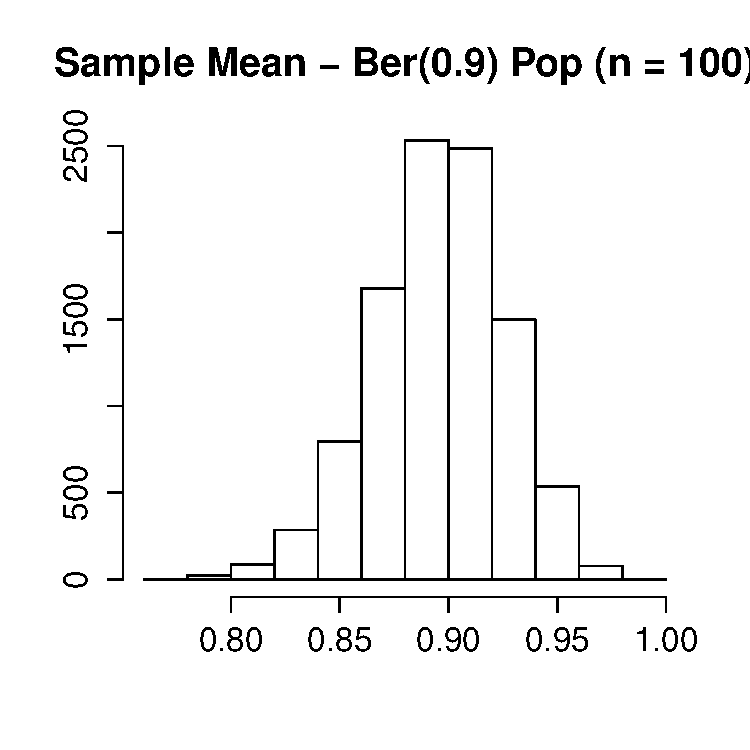
\includegraphics[scale = 0.4]{./images/xbar_bernoulli_fixed}
\end{figure}
\end{frame}
%%%%%%%%%%%%%%%%%%%%%%%%%%%%%%%%%%%%%%%%
\begin{frame}
\frametitle{Approximate 95\% CI for Population Proportion\hfill 
\includegraphics[scale = 0.05]{./images/clicker}}
39\% of 771 Voters Polled Correctly Identified Chief Justice Roberts

\begin{eqnarray*}
	\widehat{SE}(\widehat{p}) &=& \sqrt{\frac{\widehat{p}(1-\widehat{p})}{n}} = \sqrt{\frac{(0.39)(0.61)}{771}}\\ 
	&\approx& 0.018 
\end{eqnarray*}

\alert{What is the ME for an approximate 95\% confidence interval?} \pause

$$ME \approx 2 \times \widehat{SE}(\bar{X}_n) \approx 0.04$$ \pause

What can we conclude?
$$\alert{\boxed{\mbox{Approximate 95\% CI: } \; (0.35, 0.43)}}$$

\end{frame}

%%%%%%%%%%%%%%%%%%%%%%%%%%%%%%%%%%%%%%%%


\begin{frame}
\frametitle{Are Republicans Better Informed Than Democrats?}
\framesubtitle{\fbox{\href{http://www.people-press.org/files/2012/08/8-10-12-Knowledge-release.pdf}{Pew: ``What Voters Know About Campaign 2012''}}}
Of the 239 Republicans surveyed, 47\% correctly identified John Roberts as the current chief justice. Only 31\% of the 238 Democrats surveyed correctly identified him. Is this difference meaningful or just sampling variation?

\vspace{2em}
\alert{Again, assume random sampling.}


%Might be better to make a confidence interval for the proportion MINUS 0.25 to account for random guessing.

\end{frame}
%%%%%%%%%%%%%%%%%%%%%%%%%%%%%%%%%%%%%%%%
\begin{frame}
\frametitle{Confidence Interval for a Difference of Proportions}
	\begin{block}{What is the appropriate probability model for the sample?} 
$X_1, \hdots, X_n \sim \mbox{ iid Bernoulli}(p)$ independently  of $Y_1, \hdots, Y_m \sim \mbox{ iid Bernoulli}(q)$
\end{block}\pause
	\begin{block}{What is the parameter of interest?}
The difference of population proportions $p - q$
\end{block}\pause

\begin{block}{What is our estimator?}
The difference of sample proportions: $\widehat{p} - \widehat{q}$ where:
	$$\widehat{p} = \frac{1}{n}\sum_{i=1}^n X_i \quad \quad \quad	\widehat{q} = \frac{1}{m}\sum_{i=1}^m Y_i$$
\end{block}
\end{frame}

%%%%%%%%%%%%%%%%%%%%%%%%%%%%%%%%%%%%%%%%


\begin{frame}
\frametitle{Difference of Sample Proportions $\widehat{p}-\widehat{q}$ and the CLT}
\begin{block}{What We Have}
Approx.\ sampling dist.\ for \emph{individual} sample proportions from CLT:
\alert{$\widehat{p} \approx N\left(p, \widehat{SE}(\widehat{p})^2\right), \quad \widehat{q} \approx N\left(q, \widehat{SE}(\widehat{q})^2\right)$}
\end{block}\pause

\begin{block}{What We Want}
Sampling Distribution of the \emph{difference} $\widehat{p} - \widehat{q}$
\end{block}\pause

\begin{block}{Use Independence of the Two Samples}
\alert{$\widehat{p} - \widehat{q} \approx N\left( p - q, \widehat{SE}(\widehat{p})^2 +\widehat{SE}(\widehat{q})^2\right)$} \pause
$$\implies \widehat{SE}(\widehat{p} - \widehat{q}) = \pause \sqrt{\widehat{SE}(\widehat{p})^2 +\widehat{SE}(\widehat{q})^2}  = \pause  \sqrt{\frac{\widehat{p}(1-\widehat{p})}{n} + \frac{\widehat{q}(1-\widehat{q})}{m}}$$
\end{block}

\end{frame}
%%%%%%%%%%%%%%%%%%%%%%%%%%%%%%%%%%%%%%%%
\begin{frame}
\frametitle{Approx.\ 95\% CI for Difference of Population Proportions}


$$\frac{(\widehat{p} - \widehat{q}) - (p - q)}{\sqrt{\frac{\widehat{p}(1-\widehat{p})}{n} + \frac{\widehat{q}(1-\widehat{q})}{m}}} \approx N(0,1)$$
 

 

\begin{eqnarray*}
	P\left( -2 \leq  \frac{(\widehat{p} - \widehat{q}) - (p - q)}{\sqrt{\frac{\widehat{p}(1-\widehat{p})}{n} + \frac{\widehat{q}(1-\widehat{q})}{m}}}\leq 2\right) \approx 0.95 \\ \\ \\ 
	(\widehat{p} - \widehat{q}) \pm \texttt{qnorm}(1-\alpha/2) \sqrt{\frac{\widehat{p}(1-\widehat{p})}{n} + \frac{\widehat{q}(1-\widehat{q})}{m}}
\end{eqnarray*}

\end{frame}
%%%%%%%%%%%%%%%%%%%%%%%%%%%%%%%%%%%%%%%%
\begin{frame}
\frametitle{$100\times(1-\alpha)$ CI for Diff.\ of Popn.\ Proportions $(p-q)$}
$X_1, \hdots, X_n \sim \mbox{iid Bernoulli}(p)$ indep.\ $Y_1, \hdots, Y_n \sim \mbox{iid Bernoulli}(q)$
	$$(\widehat{p} - \widehat{q}) \pm \texttt{qnorm}(1-\alpha/2) \sqrt{\frac{\widehat{p}(1-\widehat{p})}{n} + \frac{\widehat{q}(1-\widehat{q})}{m}}$$
	\alert{Approximation based on the CLT. Works well provided $n,m$ large and $p,q$ aren't too close to zero or one.}
\end{frame}
%%%%%%%%%%%%%%%%%%%%%%%%%%%%%%%%%%%%%%%%


\begin{frame}
\frametitle{ME for approx.\ 95\% for Difference of Proportions}

\footnotesize
\fbox{47\% of 239 Republicans vs.\ 31\% of 238 Democrats identified Roberts}
\singlespacing
\begin{columns} 
	\column{0.5\textwidth}
	\begin{block}{Republicans}
		\begin{eqnarray*}
			\widehat{p} &=& 0.47\\
			n &=& 239\\  \pause
			\widehat{SE}(\widehat{p}) &=&\sqrt{ \frac{\widehat{p}(1-\widehat{p})}{n}} \approx 0.032 \\ \pause
		\end{eqnarray*}
	\end{block}
	
	\column{0.5\textwidth}
		\begin{block}{Democrats}
		\begin{eqnarray*}
			\widehat{q} &=& 0.31\\
			m &=& 238\\  \pause
			\widehat{SE}(\widehat{q}) &=& \sqrt{\frac{\widehat{q}(1-\widehat{q})}{m}} \approx 0.030\\ \pause
		\end{eqnarray*}
	\end{block}
\end{columns}

\begin{block}{Difference: (Republicans - Democrats)}
	\begin{eqnarray*}
		\widehat{p} - \widehat{q} &=& 0.47 - 0.31 = 0.16\\ \pause
		\widehat{SE}(\widehat{p} - \widehat{q}) &=& \sqrt{\widehat{SE}(\widehat{p})^2 + \widehat{SE}(\widehat{q})^2} \approx 0.044  \pause \implies ME \approx 0.09 \pause 
	\end{eqnarray*}
	$$\alert{\boxed{\mbox{Approximate 95\% CI} \quad (0.07, 0.25)}} \quad \mbox{What can we conclude?}$$
\end{block}

\end{frame}
%%%%%%%%%%%%%%%%%%%%%%%%%%%%%%%%%%%%%%%%



\end{document}